\documentclass[]{article}
\usepackage[utf8]{inputenc} % accented characters in input
\usepackage[portuguese]{babel}
\usepackage{amssymb}
\usepackage{amsmath}
\usepackage{graphicx}
\usepackage{float}
\usepackage{blindtext}
\usepackage{enumitem}
\usepackage{xcolor}
\usepackage{titlesec}
\usepackage{multicol}

\newtheorem{definition}{Definição}[section]
\newtheorem{theorem}{Teorema}[section]
\newtheorem{algorithm}{Algoritmo}[section]


\renewcommand{\theenumi}{\Alph{enumi}}
\newcommand{\R}{\mathbb{R}}


%opening
\title{Agrupamento espectral}
\author{Piero Kauffmann (8940810)}

\begin{document}

\maketitle

\section{Introdução e definições}

Este capitulo introduz algumas definições sobre grafos valorados não-direcionados, que serão essenciais para a formulação do algoritmo de agrupamento espectral. As importantes matrizes de adjacência e de grau de um grafo são definidas abaixo

% Definição grafos

\begin{definition}{Matriz de adjacências}

\vspace{0.1cm}

Seja $G = (V, E, W)$ um grafo valorado com vértices $V = \{v_1, ..., v_n\}$

Definimos a matriz de adjacências $W_{nxn}$ como a matriz cujos elementos $w_{ij}$ satisfazem


\[
    w_{ij}= 
\begin{cases}
    0, & \text{se } i \neq j \text{ e } \{i,j\} \not\in E\\
    s_{ij}, & \text{se } i = j \text{ ou } \{i,j\} \in E\\

\end{cases}
\]

Onde $s_{ij} > 0 $

\end{definition}

\begin{definition}{Grau do grafo}\\
\vspace{0.1cm}
Seja $G = (V, E, W)$ um grafo valorado com vértices $V = \{v_1, ..., v_n\}$

\vspace{0.1cm}

A matriz $D_{nxn} = diag(d_1, ..., d_n)$, é a matriz de grau do grafo $G$ se 
$$d_i = \sum_{j = 1}^{n} w_{ij}, \text{ para } i = 1, ..., n$$

\end{definition}

\vspace{.3cm}

A matriz de adjacências ($W$) de um grafo carrega significados muito importantes. O principal deles é a informação sobre as arrestas do grafo, que podem ser inferidas pelos valores não-nulos da matriz. É possível codificar informações de similaridade ou dissimilaridade entre os vértices do grafo por meio dos pesos $s_{ij}$. Por razões de simplicidade, neste trabalho usaremos os pesos unitários ($s_{ij} \in \{0, 1\}$) para medir similaridade.

\newpage

\begin{definition}{Laplaciano \textit{Random Walk}}\\

\vspace{0.2cm}

Seja $G = (V, E)$ um grafo valorado com vértices $V = \{v_1, ..., v_n\}$ e matriz de adjacências ponderada $W$. Definimos 

\vspace{0.1cm}

$$L_{rw} = I_n - D^{-1}W$$

\end{definition}

\vspace{0.1cm}

Verificamos da definição do Laplaciano que $L_{rw} = I - P$, onde $P = D^{-1}W$ é a matriz de transições de um passeio aleatório no grafo.

O Laplaciano carrega ingormações e propriedades importantes sobre o grafo. Algumas delas são listadas abaixo:


\begin{itemize}
\item $L_{rw}$ é simétrica e semi positiva definida

\vspace{.1cm}

\item O número de autovalores iguais a zero de $L_{rw}$ é igual ao número de conjuntos de vertices disjuntos não conexos.

\begin{figure}
\hspace*{2.3cm}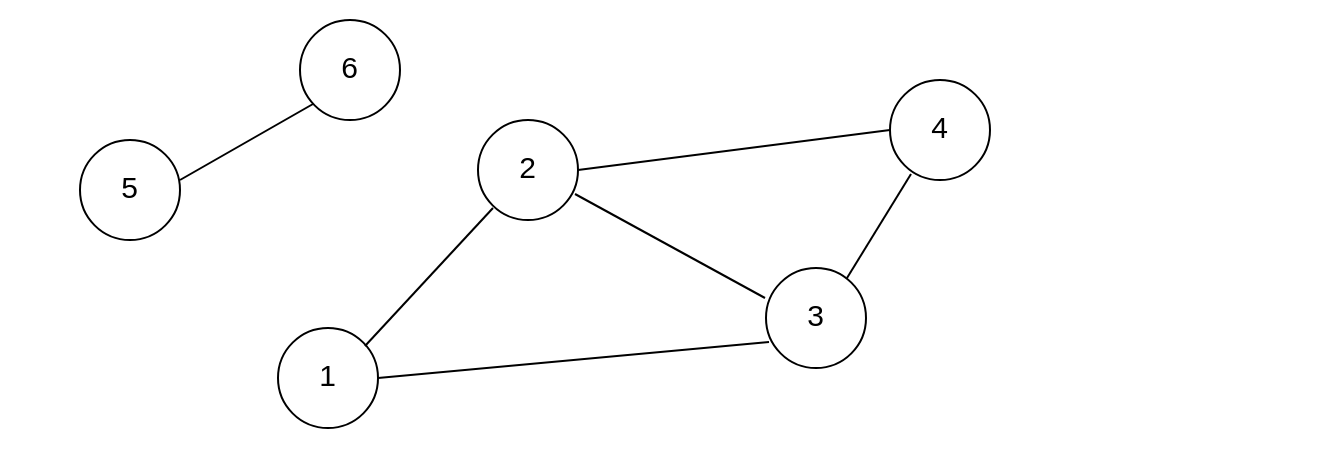
\includegraphics[scale=0.15]{grafo2_pequeno}
\caption{Exemplo de um grafo cujo Laplaciano $L_{rw}$ possui dois autovalores nulos}
\end{figure}

\item  Se $u$ é um autovetor da matriz de transição $P$ do passeio aleatório $\Leftrightarrow$ $u$ é autovetor de $L_{rw}$

\end{itemize}

A segunda propriedade é importante pois está fortemente relacionada a presença de grupos aparentes no grafo. Um fato observável é que autovalores próximos a zero, indicam a presença de grupos quase não conexos também. A terceira propriedade será útil para compreender a construção do modelo em termos de passeios aleatórios no grafo.

\newpage

\section{Construção do grafo de similaridade a partir de pontos no $\R^p$}

\begin{figure}
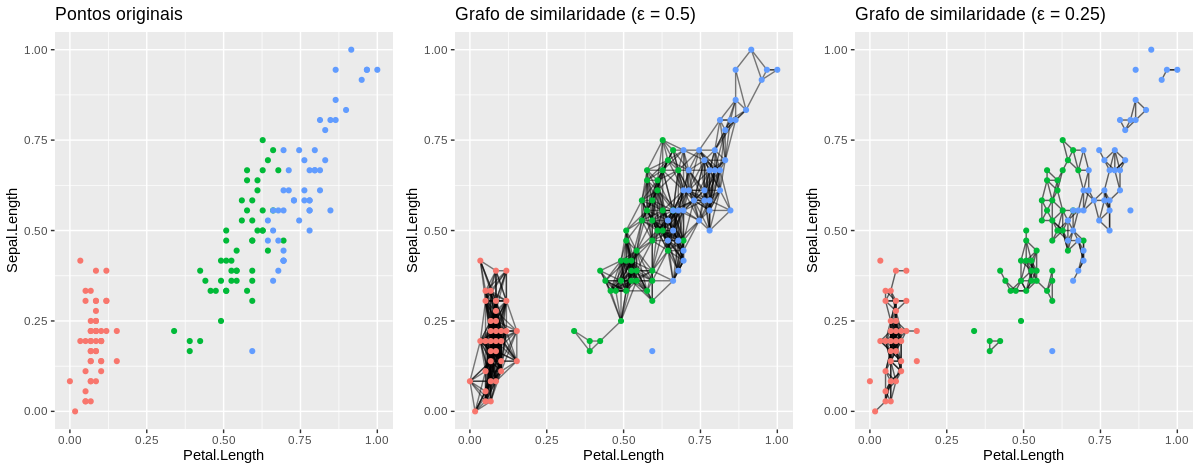
\includegraphics[scale=0.45]{epsilon_similarity}
\caption{Método da $\epsilon$-vizinhança aplicado ao conjunto de dados \textit{iris} representados em duas variáveis, as cores representam as três espécies de plantas.}
\end{figure}

Na literatura, existem três métodos mais utilizados para construir grafos de similaridade a partir de uma amostra $x_i, ..., x_n \in \R^p$. 

\begin{itemize}
\item Método da $\epsilon$-vizinhança
\begin{itemize}
\item Todos os pares de pontos no conjunto de dados cujas distâncias sejam menores que $\epsilon$ são conectados
\end{itemize}

\item Método dos $k$-vizinhos mais próximos
\begin{itemize}
\item Cada ponto no conjunto de dados é conectado aos seus $k$ vizinhos mais próximos
\end{itemize}

\item Método da função de similaridade


\begin{itemize}
\item Todos os pontos são conectados entre si, mas as similaridades entre cada par de pontos $w_{ij}$ é obtida segundo uma função \textit{Kernel} de similaridade $s: \R^p \times \R^p \rightarrow [0,1]$
\item Uma escolha comum é $ s(x_i, x_j) = exp(-\parallel x_i - x_j\parallel^2/(2\sigma^2))$
\end{itemize}

\end{itemize}

A Figura 2 é um exemplo da aplicação do método da $\epsilon$-vizinhança para a construção do grafo de similaridades. O parâmetro $\epsilon$ controla o nível de detalhamento das conexões formadas. Um valor baixo para $\epsilon$ (quadro da direita) pode resultar em um grafo com muitos sub grupos não conexos entre si, enquanto um valor muito elevado para o parâmetro pode resultar em um grafo que associa pontos muito distantes entre sí.

\vspace{0.3cm}

\section{Intuição e justificativa do algoritmo}


%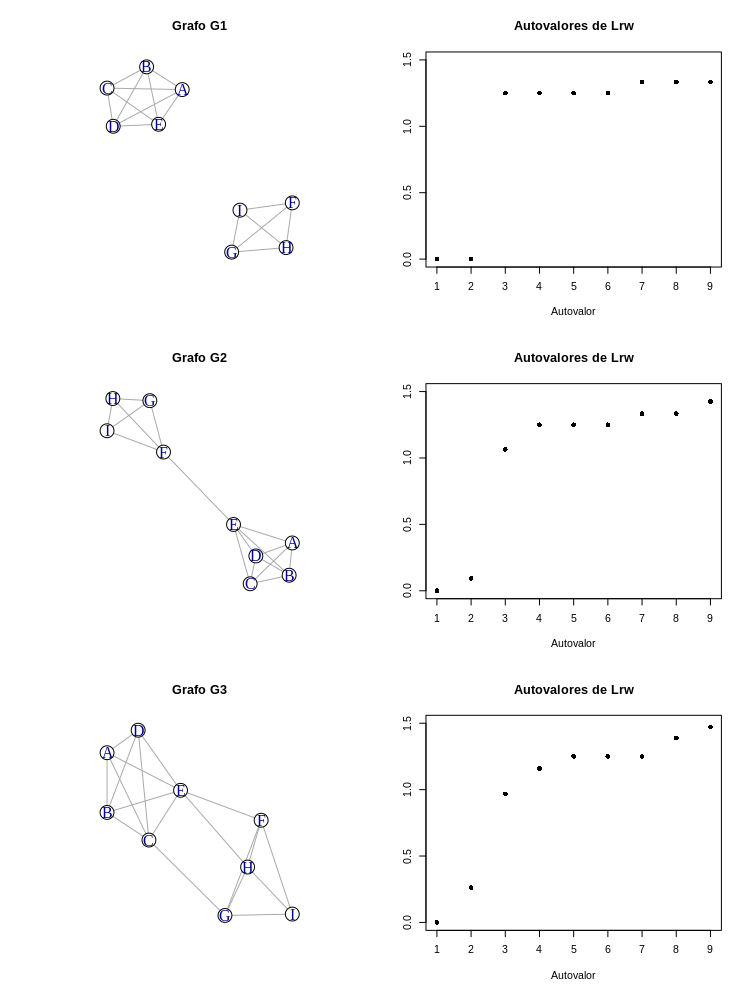
\includegraphics[scale=0.65]{grafo_just}





Sejam $A_1, ..., A_k \subset V$ conjuntos disjuntos de vértices do grafo G. 

\vspace{0.3cm}

Definimos distribuição $\pi^{A}$ como 

$$\pi^{A}_i = \begin{cases} 1/|A|, & \text{se } i \in A \\ 0, & \text{caso contrário}\end{cases}$$

\vspace{0.5cm}

Procuramos $\pi^A$ que minimize a probabilidade do passeio aleatório sair ou entrar no conjunto $A$ , $C_A = P(A|A^C) + P(A^C|A)$

\vspace{0.5cm}

Pode ser provado que os k-primeiros autovetores de $L_{rw}$ são uma solução aproximada para o problema, relaxando-se algumas suposições sobre $\pi^A$.

Uma interpretação possível está ligada com a distribuição estacionária $\pi$ do passeio aleatório no grafo. É conhecido da teoria de matrizes estocásticas que os autovalores (com exceção do primeiro) estão relacionados com a velocidade de convergência a distribuição estacionária partindo-se de uma distribuição inicial. Fazendo uma ponte com a matriz $L_{rw}$, uma interpretação é que os autovetores são representações associadas a distribuições no grafo e seus autovalores associados indicam a velocidade de convergência desta distribuição à distribuição estacionária $\pi$. Autovalores mais baixos indicam tempos maiores para a distribuição da cadeia convergir.

O exemplo na Figura 3 demonstra o efeito da estrutura do grafo nos autovalores. O tempo de convergência da cadeia é maior quando partimos de uma distribuição $\pi^A$ em um grafo muito particionado, pois o passeio aleatório demora para explorar a região $A^C$. Um exemplo extremo é quando o grafo possui dois subgrupos não conexos, o que indicaria que o tempo de convergência é infinito, isto é, $\lambda_2 = 0$.

\begin{figure}
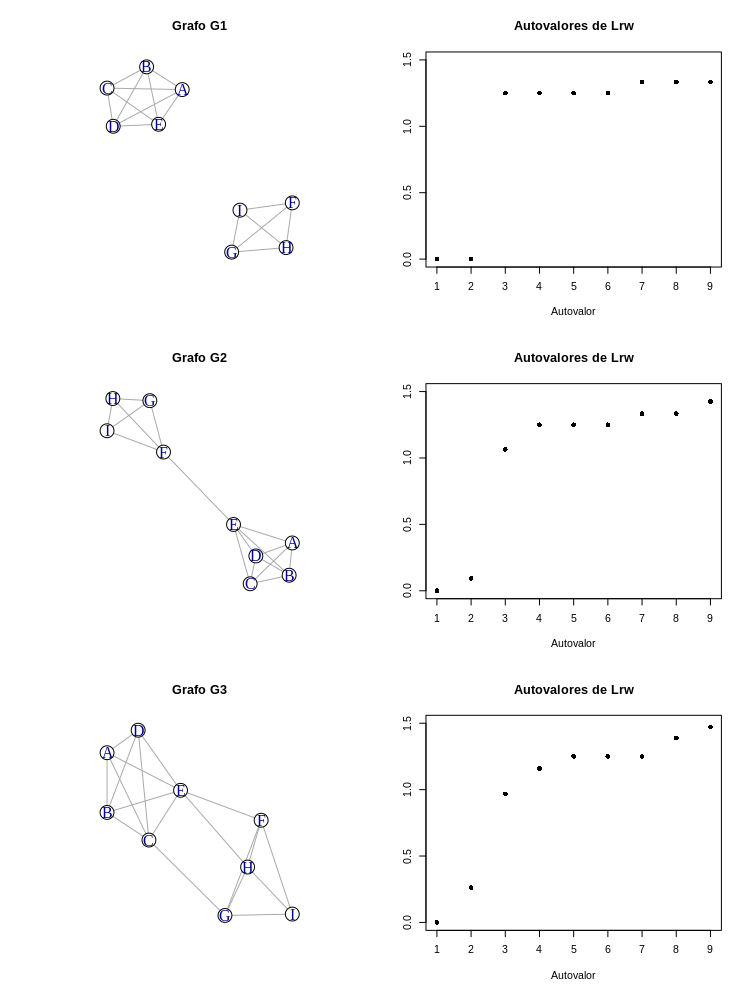
\includegraphics[width=13cm,height=16cm]{grafo_just}
\caption{De cima para baixo, o comportamento do segundo autovalor varia de acordo com a conectividade entre os dois grupos de vértices \{A, B, C, D, E\} e \{F, G, H, I\}}.
\end{figure}

\newpage
\section{Algoritmo}

\begin{enumerate}
\item Criar um grafo de similaridades entre os pontos do conjunto de dados 

\begin{itemize}
\item Usando o métodos da $\epsilon$-vizinhança, por exemplo

\end{itemize}

\vspace{0.5cm}
\item Calcular o Laplaciano $L_{rw} = I - D^{-1}W = I - P$

\vspace{0.5cm}

\item Extrair os $k$-primeiros autovetores de $L_{rw}$, excluindo-se o primeiro autovetor

\vspace{0.5cm}

\item Aplicar o método das K-médias na matriz de dados dos $k$-autovetores extraidos

\end{enumerate}

\vspace{1cm}

\subsection{Exemplo de aplicação do algoritmo}

Utilizando o conjunto de dados criado por Jain \& Law (2006) o algoritmo foi aplicado. Os dados originais foram transformados em um grafo de similaridades usando o método da $\epsilon$-vizinhança, com $\epsilon = 4$. 

\vspace{1cm}
\begin{figure}[h!]
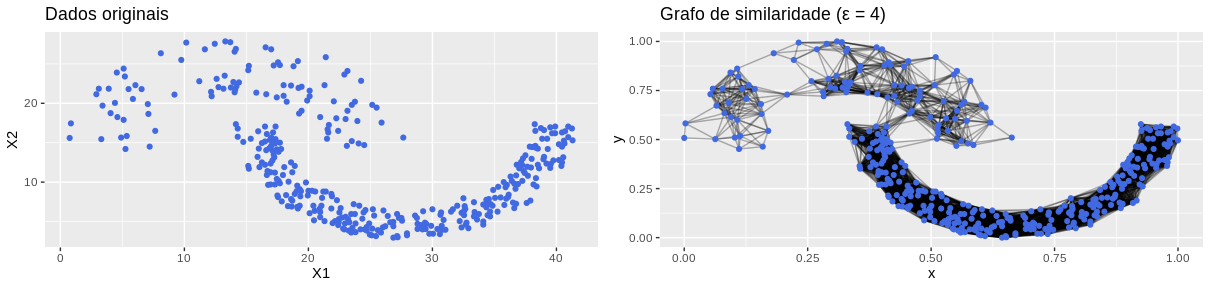
\includegraphics[width=13cm, height = 4.5cm]{horse}
\end{figure}

Após a criação do grafo de similaridade, foi extraido o segundo autovetor do grafo para aplicação do método das K-médias (K = 2)

\newpage

\vspace{1cm}
\begin{figure}[h!]
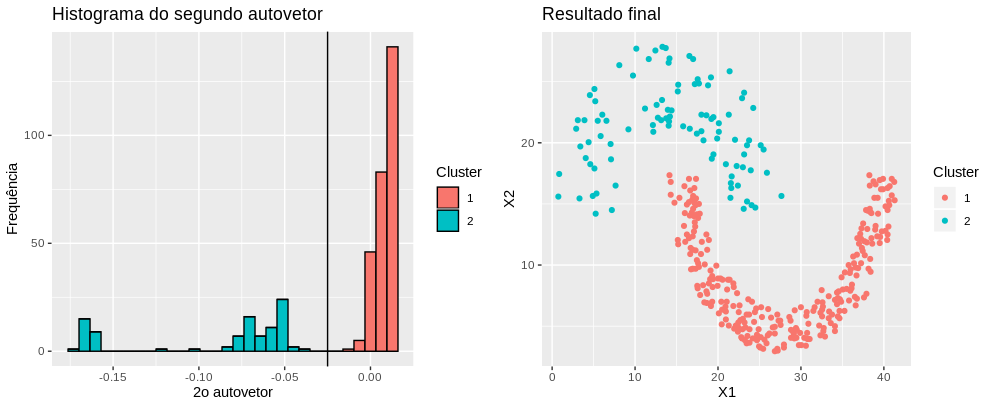
\includegraphics[width=13cm, height = 4.5cm]{final}
\end{figure}

\vspace{0.5cm}

Os resultados mostraram a separação dos dois grupos mais evidentes utilizando o segundo autovetor.

%###################

\newpage

\section{Referências}

\vspace{0.2cm}

\hspace{0.37cm} LUXBURG, U. (2007); “\textbf{A Tutorial on Spectral Clustering}".\\

LOVÀSZ, L. (1993); “\textbf{Random walks on graphs: A Survey}".\\

JAIN, A. \& LAW, M. (2006); “\textbf{Data Clustering: A User’s Dilemma}".\\



\end{document}